\documentclass[fr,license=none]{../../../eplsummary}

\usepackage{float}
\usepackage{rotating}

\usepackage{../../../eplcode}
\lstset{language={Java},morekeywords={for}}

\hypertitle{Méthodes de conception de programmes}{6}{LINGI}{1122}
{Croix Benjamin\and Wynen Maxence}
{Charles Pecheur}

\part{Preuves de programme}
\section{Introduction}

\subsection{Science de la programmation}
Le \textbf{déboguage} : programmer, tester, corriger, jusqu'à ne plus trouver d'erreurs. C'est \textbf{inefficace} en tant que méthodologie. Ca ne permet pas d'établir que le programme est \textbf{correct}. Ce n'est pas fiable pour détecter que le programme n'est \textbf{pas correct}. Chaque test réussi \textbf{augmente notre confiance} en la justesse de l'algorithme, mais on n'est \textbf{jamais sûr}.\\

Le \textbf{déboguage} et le \textbf{ test} sont donc incertain pour établir la correction et pour trouver les erreurs mais surtout, inutile comme base de \textbf{construction} de programmes.\\

Une \textbf{science de la programmation} sert à \textbf{spécifier} les programmes, \textbf{vérifier} les programmes par rapport à leurs spécifications et \textbf{construire} les programmes sur base de leurs spécifications.


\subsection{Problème, solution et preuve}
$\bullet$\textbf{Théorie du problème}:
Dans la théorie du problème, on définit les \textbf{structures}, les \textbf{opérations} et \textbf{caractéristiques} ainsi que les \textbf{propriétés utiles}. On définit également les \textbf{cas particuliers}.\\

$\bullet$\textbf{Solution}:
Dans la solution, on détermine "\textbf{comment faire ?}". On généralise le résultat désiré. On définit une situation initiale et une situation finale pour ensuite définir une itération entre ces 2 situations.\\

$\bullet$\textbf{Preuve}:
La \textbf{correction} assure que si les données satisfont les pré-conditions, alors les résultats satisfont les post-conditions.\\
La \textbf{terminaison} assure que si les données satisfont les pré-conditions, alors le programme se termine.\\
La \textbf{correction partielle} assure que si les données satisfont les pré-conditions, et si le programme se termine, alors les résultats satisfont les post-conditions.\\
Correction totale $\equiv$ Correction partielle ET Terminaison
\\ \vspace{1,5mm}\\
On prouve la terminaison grâce au \textbf{variant}. Il \textbf{diminue} à chaque itération et est toujours \textbf{positif ou nul}. Le nombre d'itérations est donc fini.\\
On prouve la correction partielle grâce à l'\textbf{invariant}. Si les pré-conditions sont vraies initialement, alors l'invariant est vrai à l'entrée dans la boucle.\\ Si l'invariant est vrai avant une itération de la boucle, alors l'invariant est vrai après l'itération.\\ Si l'invariant est vrai à la sortie de la boucle, alors les post-conditions sont vraies finalement.\\ \vspace{1,5mm}\\
La preuve sur l'itération est une récurrence. Il y a une \textbf{cas de base}, un \textbf{cas inductif} et une \textbf{conclusion}.\\

$\bullet$\textbf{Représentation}:
La représentation cherche à trouver la meilleure représentation pour les données, le problème, la solution et la preuve.
\subsection{Spécifier des programmes}
Les \textbf{assertions de programme} sont des propositions vraies à un point du programme.\\

\textbf{Assertion}: [ p ] $\equiv $ en ce point, p est vrai, avec p comportant des \textbf{variables du programme}\\

$\bullet$\textbf{Triplet de Hoare}:
[P] S [Q] $\equiv$ \textbf{triplet de Hoare}, \\ avec pré-condition P, programme S et post-condition Q.\\

[P] S [Q] est une \textbf{proposition logique}, valide ou invalide. [P]S[Q] est valide ssi : \\- \hspace{5mm} \textbf{Si P est vraie avant} d'exécuter S\\- \hspace{5mm} \textbf{Alors} l'exécution de S \textbf{se termine}\\- \hspace{5mm} \textbf{Et Q est vraie après} l'exécution de S.\\ \hspace{5mm}
C'est une \textbf{correction totale}, S réalise Q sous l'assomption de P.\\

$\bullet$\textbf{Variables auxiliaires}:
Les variables auxiliaires ne sont pas des variables du programme. Elles sont rigides et donc ne change pas au cours de l'exécution.\\

$\bullet$\textbf{Conséquence}:
La conséquence est un connecteur logique qui peut lier deux pré- ou post-conditions ensemble.\\

[Cond1] $\Rightarrow$ [Cond2], avec Cond1 plus contraignante que Cond2\\

Dans le cas de la pré-condition, elle crée un \textbf{renforcement} de la pré-condition. On va rajouter une pré-condition plus contraignante et précise au-dessus de la condition actuelle.
Dans le cas de la post-condition, elle crée un \textbf{affaiblissement} de la post-condition. On va rajouter une post-condition moins contraignante en dessous de la condition actuelle. \\

La règle de conséquence est la suivante : \textbf{Si P $\Rightarrow$ Q, alors [P][Q]}
\section{Programmes séquentiels}
\subsection{Affectations}
\textbf{\textit{Affectation} : V:=E;}\\ V une variable et E une expression.\\ 
Affectation simultanée: $V_1,...,V_n := E_1,...,E_n$;\\

$\bullet$\textbf{Axiome l'affectation :\\ $\quad$ [Q[V:=E]] V:=E;[Q]}\\
La notation [Q[V:=E] définit la condition [Q] où toutes les occurrences de V sont remplacées par E.\\
\textit{ou}\\
\textbf{[Q[E]]V:=E;[Q[V]]}\\

$\bullet$\textbf{Prouver et construire}:
La construction de l'affectation se fait autour de la conservation de l'invariant avant et après l'affectation.
\vspace{5mm}
\subsection{Séquences}
\textbf{\textit{Composition séquentielle} S1 S2},\\
elle est associative : \{S1 S2\} S3 = S1 \{S2 S3\} = S1 S2 S3\\

$\bullet$\textbf{Règle}:
Si [P]S1[R] et [R]S2[Q], Alors [P] S1 S2 [Q]\\
La preuve en arrière part de Q pour calculer ensuite R et puis P. La preuve en avant fait le chemin inverse.\\

$\bullet$\textbf{Prouver et construire}:
Pour construire une séquence, on invente R, S1 ou S2 et on calcule ensuite les deux autres.\\

$\bullet$\textbf{Axiome de l'instruction vide :  [Q] \{\}[ Q ]}\\
Avec la règle de conséquence:\\
Si [P] $\Rightarrow$ Q alors [P][Q]\\
Si [P]$\Rightarrow$ [Q] alors [P] [Q] \{\} [Q] \textit{ou} [P] \{\} [P] [Q] \textit{ou} [P] \{\} [Q]\\
Aussi \{\}S = S = S\{\}
\vspace{5mm}
\subsection{Conditionnelles}
\textbf{\textit{Conditionnelle} : if C\{S1\} else \{S2\}}, avec if C \{S1\} $\equiv$ if C \{S1\} else \{\} \\

$\bullet$\textbf{Règle}:\\
- Règle de la conditionnelle en \textbf{avant} :\\
.[P] if C then S1 else S2 fi [Q] \\si et seulement si  [P $ \wedge$ C] S1 [Q] et [P $\wedge$ $\neg$C] S2 [Q]\\\vspace{2,5mm}\\
- Règle de la conditionnelle en \textbf{arrière} :\\
Si [P1] S1 [Q] et [P2] S2 [Q] \\ Alors [(C $\Rightarrow$ P1) $\wedge$ ($\neg$C $\Rightarrow$P2)] if C \{S1\} else \{S2\} [Q]
\subsection{Itérations}
\textbf{\textit{Itération}: while C \{S\}}\\
Deux nouvelles assertions sont nécessaires : l'invariant pour la correction partielle et le variant pour la terminaison.\\

$\bullet$\textbf{Invariant et variant}:\\

Pour la correction \textbf{partielle}, on utilise l'invariant \textbf{I}.\\
Si [I $\wedge$ C] S [I] \\Alors [I] while C \{S\} [I $\wedge$ $\neg$C]\\
Pour prouver [P] while C \{S\} [Q], il faut trouver un invariant I tel que :\\
P $\Rightarrow$ I et (I$\wedge$ $\neg$C) $\Rightarrow$ Q\\

Pour la correction \textbf{totale}, on utilise, en plus de l'invariant, le variant \textbf{V}\\
Si I $\Rightarrow$ V $\geq$ 0 \\ et [I $\wedge$ C $\wedge$ V = $v_0$] S [I $\wedge$ V < $v_0$] \\Alors [I] while C \{S\} [I $\wedge$ $\neg$C]
\section{Induction}

\subsection{Notions}
Un \textbf{raisonnement inductif} est le fait d'inférer une règle générale à partir d'observations particulières par opposition à un raisonnement déductif. Dans le cadre de l'induction expérimentale, on part d'observations expérimentales et on en déduit un modèle général. C'est une méthode incertaine, ce n'est qu'une accumulation d'évidences.\\

L'\textbf{induction mathématique}, quant à elle, part de propriétés de cas particuliers pour en déduire une propriété générale. Cette méthode est certaine car prouvée.\\

Ensembles inductifs : ex. un naturel est 0 ou le successeur d'un naturel.\\

Définitions inductives : 0!=0, (n+1)!=(n+1)xn!

\subsubsection{Preuve calculatoire d'égalité}
On prouve $E_0=E_n$
\begin{align*}
	E_0 &= E_1 [w_1]\\
	&= E_2 [w_2]\\
	&= ...\\
	&= E_n [w_n]
\end{align*}
E sont des expressions et w sont des indices (explications, justifications). Chaque $w_i$ justifie pourquoi $E_i = E_{i+1}$
\subsection{Induction simple}
Soit P[n] une propriété dépendant de n.\\
\textbf{Si\\ $\bullet$ P[0] est vrai et \\ $\bullet$ si P[n] est vrai alors P[n+1] est vrai \\ Alors P[n] est vrai pour tout n}\\
(P[0] $\wedge$ ($\forall$n : P[n] $\Rightarrow$ P[n+1])) $\Rightarrow$ $\forall$n : P[n]\\

Induction simple $\equiv$ récurrence !
\subsubsection{Induction simple à partir de k}
Soit P[n] une propriété dépendant de n.\\
Si\\ $\bullet$ P[k] est vrai et \\ $\bullet$ si P[n] est vrai alors P[n+1] est vrai pour tout n $\geq$ k \\ Alors P[n] est vrai pour tout n$\geq$ k\\

(P[k] $\wedge$ ($\forall$n$\geq$ k : P[n] $\Rightarrow$ P[n+1])) $\Rightarrow$ $\forall$n $\geq$ k : P[n]\\

Induction simple $\equiv$ récurrence !
\subsubsection{Induction d'ordre 2}
Soit P[n] une propriété dépendant de n.\\
Si\\ $\bullet$ P[0] est vrai et P[1] est vrai \\ $\bullet$ si P[n] et P[n+1] sont vrais alors P[n+2] est vrai\\ Alors P[n] est vrai pour tout n\\

(P[k] $\wedge$P[1] $\wedge$ ($\forall$n: P[n] $\wedge$ P[n+1] $\Rightarrow$ P[n+2])) $\Rightarrow$ $\forall$n  : P[n]\\

\subsubsection{Induction d'odre k}
Soit P[n] une propriété dépendant de n.\\
Si\\ $\bullet$ P[0] est vrai et ... et P[k-1] est vrai \\ $\bullet$ si P[n] et ... et P[n+k-1] sont vrais alors P[n+k] est vrai\\ Alors P[n] est vrai pour tout n\\

(P[k] $\wedge$ ... $\wedge$ P[1] $\wedge$ ($\forall$n: P[n] $\wedge$ ... $\wedge$ P[n+1] $\Rightarrow$ P[n+2])) $\Rightarrow$ $\forall$n  : P[n]\\

\subsubsection{Preuve calculatoire d'implication}
On prouve $P_0\Leftarrow P_n$
\begin{align*}
P_0 &\Leftarrow P_1 [w_1]\\
&\Leftarrow P_2 [w_2]\\
&\Leftarrow ...\\
&\Leftarrow P_n [w_n]
\end{align*}
P sont des assertions (propositions, formules) et w sont des indices (explications, justifications). Chaque $w_i$ justifie pourquoi $E_i \Leftarrow E_{i+1}$\\
On peut avoir des $\Leftrightarrow$ (si P $\Leftrightarrow$ P' alors P $\Leftarrow$ P')
\subsubsection{Preuve calculatoire d'inégalité}
On prouve $E_0 \geq E_n$
\begin{align*}
E_0 &\geq E_1 [w_1]\\
&\geq E_2 [w_2]\\
&\geq ...\\
&\geq E_n [w_n]
\end{align*}
E sont des expressions et w sont des indices (explications, justifications). Chaque $w_i$ justifie pourquoi $E_i \geq E_{i+1}$\\
On peut avoir des = (si E = E' alors E $\geq$ E').\\
On peut avoir des $>$ (si E $>$ E' alors E $\geq$ E').
\vfill

\subsection{Induction complète}
Soit P[n] une propriété dépendant de n.\\
\textbf{Si:\\ si P[k] est vrai pour k $<$n alors P[n] est vrai \\  Alors P[n] est vrai pour tout n}\\

\textbf {($\forall$n :($\forall$ k $<$ n: P[k]) $\Rightarrow$ P[n])) $\Rightarrow$ $\forall$n : P[n]}\\

Il n'y a \textbf{pas de cas de base}, P[0] est couvert par le cas inductif. Mais la définition de P[n] peut avoir un cas particulier pour n=0 ou 1 ou autre...\\

$\bullet$\textbf{Induction complète et variants}:
La règle de l'itération de correction totale $\equiv$ une induction complète sur le variant.
\subsection{Induction bien-fondée}
Une \textbf{relation} $\prec$ est \textbf{bien-fondée} (sur un ensemble W) ssi il n'existe pas de chaîne décroissante infinie (dans l'ensemble W). Ssi tout sous-ensemble de W a au moins un élément minimal.\\
$ \nexists \; x_1,x_2,x_3,... \in W : x_1 \succ x_2 \succ x_3 \succ ... $ et
$\forall X \subseteq W : \exists x \; \in X : \forall y \in X : y \nprec x $\\

Une relation bien-fondée est:\\
$\bullet$ \textbf{Irréflexible :} $x \nprec x$\\
$\bullet$ \textbf{Asymétrique :} $x \prec y \Rightarrow y \nprec x$\\
$\bullet$ \textbf{Pas nécessairement transitive :} on peut avoir $x \prec y, y \prec z, x \nprec z$, il n'y a donc pas nécessairement d'ordre.\\
$\bullet$ \textbf{Pas nécessairement totale :} on peut avoir $x \neq y, x \nprec y, y \nprec x$\\

\subsubsection{Principe d'induction bien-fondée}
Pour une relation ($\prec$) bien-fondée dans W\\
Si\\
si P[y] est vrai pour tout y $\prec$ x dans W \\ alors P[x] est vrai\\
Alors P[x] est vrai pour tout x dans W.\\

\textbf{Induction complète} $\equiv$ \textbf{induction bien-fondée} sur l'ordre ($<$) des entiers naturels.

\subsubsection{Preuve calculatoire d'inégalité stricte}
On prouve $E_0 > E_n$
\begin{align*}
E_0 &\geq E_1 [w_1]\\
&\geq E_2 [w_2]\\
&> ...\\
&\geq ...\\
&\geq E_n [w_n]
\end{align*}
E sont des expressions et w sont des indices (explications, justifications). Chaque $w_i$ justifie pourquoi $E_i \geq E_{i+1}$\\
On peut avoir des = (si E = E' alors E $\geq$ E').\\
Il faut au moins un $>$ (si E $\geq$ E'' $>$ E''' $\geq$ E' alors E $>$ E').

\subsubsection{Structures}
Une structure est composée de  structures, de formules, de phrases, de programmes, de \textbf{termes}. Toutes les valeurs sont à \textbf{construction finie}.\\

Une \textbf{relation de sous-terme} strict se définit comme:\\
t $<$ t'\\
ssi t est un \textbf{sous-terme strict} de t'\\
ssi t \textbf{apparait dans} et est \textbf{différent de} t'\\
t $<$ t' $\Leftrightarrow$ t' = u[t] $\wedge$ t' $\neq$ t\\
La relation de sous-terme est \textbf{bien-fondée} !
\subsubsection{Principe d'induction structurale}
Induction bien-fondée sur les sous-termes $\equiv$ \textbf{induction structurale}\\ \vspace{0.5mm}\\
Si\\ si P[y] est vrai pour tout sous-terme y de x\\ alors P[x] est vrai\\ Alors P[x] est vrai pour tout terme x

\subsection{Résumé}
$\bullet$ induction simple : P[0], P[n] $\Rightarrow$ P[n+1] \\

$\bullet$ induction complète: ($\forall$ k$<$n : P[k]) $\Rightarrow$ P[n]\\

$\bullet$ induction bien-fondée: ($\forall$ k$\prec$n : P[k]) $\Rightarrow$ P[n]\\

$\bullet$ induction structurale: ($\forall$ k sous-terme de n : P[k]) $\Rightarrow$ P[n]\\

\section{Preuves de programmes}

Pour prouver un programme, il faut le décomposer en \textbf{chemins simples} et utiliser des \textbf{assertions inductives}, càd qui sont conservées sur chaque chemin, et des \textbf{ensembles bien-fondés}, càd que les variants diminuent sur chaque chemin de boucle.
\subsection{Chemins simples}
Une \textbf{position} du programme est un point avant, après ou entre des instructions successives du programme. \textit{Dénotation:} @label\\

Un \textbf{chemin} est une séquence exécutable d'instructions du programme entre 2 positions.\\

Un \textbf{chemin simple} est un chemin qui ne passe pas deux fois par la même instruction, càd par des positions différentes sauf éventuellement quand la fin correspond au début dans le cas d'un cycle.\\

Un ensemble de \textbf{points de coupe} est un ensemble de positions du programme tel que \textbf{toutes les boucles contiennent au moins un point de coupe}. Les chemins entre les points de coupe sont des chemins simples.\\ \vspace{5mm}\\

$\bullet$ L'instruction \textbf{assume}: les conditions dans les instructions du programme deviennent des assomptions dans les chemins simples.\\
@L1 if C \{S1\} else \{S2\} @L2\\
$.\quad \rightarrow$ @L1 assume C; S1 @L2\\
$.\quad \quad$ @L1 assume $\neg$C; S2 @L2\\
@L1 while C \{S\} @L2\\
$.\quad \rightarrow$ @L1 assume C; S @L1\\
$.\quad \quad$ @L1 assume $\neg$C; @L2\\ 

\textbf{assume C} $\equiv$ le reste de l'exécution ne s'exécute que si C est vrai.\\
Règle de l'assume avant: [P] assume C; [P $\wedge$ C]\\
Règle de l'assume arrière: [C $\Rightarrow$ Q] assume C; [Q]\\
On assume que C est vrai $\equiv$ on ignore les exécutions où C est faux.\\ \vspace{5mm}\\

$\bullet$ L'instruction \textbf{assert}: assert C $\equiv$ en cette position, C est vrai\\
Règle de l'assert en version avant : \textbf{Si [P] $\Rightarrow$ C alors [P] assert C; [P $\wedge$ C]}\\
Règle de l'assert en version arrière : \textbf{[C $\wedge$ Q] assert C; [Q]}\\
On affirme que C est vrai, on doit donc le prouver sur toutes les exécutions.\\ \vspace{5mm}\\

Un chemin simple est une séquence d'instructions suivantes:\\
$\bullet$ Affectation V:=E;\\
$\bullet$ Assomption assume C;\\
$\bullet$ Assertion assert C;
\vfill
\subsection{Calcul WP}
La \textbf{plus faible pré-condition} de S (un chemin simple) pour Q : wp(S,Q).\\
Q est vrai après le chemin simple S ssi wp(S,Q) est vrai avant S $\equiv$ \textbf{[P] S [Q] ssi P $\Rightarrow$ wp(S,Q)}\\
Pre $\Rightarrow$ wp(S,Post)
\begin{align*}
	wp(V:=E;, Q) &= Q[V:=E]\\
	wp(assume C;, Q) &= C \Rightarrow Q\\
	wp(assert C;, Q) &= C \wedge Q\\
	wp(S1 S2, Q) &= wp(S1, wp(S2,Q))
\end{align*}
\subsection{Méthodes des assertions inductives}
Pour prouver la \textbf{ correction partielle} de $[P] S [Q]$, il faut choisir un ensemble de \textbf{points de coupe} $L_1,...,L_n$ au début, à la fin du programme et dans les boucles. Ensuite, il faut associer une \textbf{assertion}(pré,post,invariants) $P_i$ à chaque point de coupe $L_i$. Pour chaque \textbf{chemin simple} @$L_i S$ @$L_j$, il faut \textbf{prouver} $[P_i] S [P_j]$\\

Si $[P_i] S_{ij}[P_j]$ est  valide pour tout \textbf{chemin simple} @$L_i S_{ij}$ @$L_j$,\\
alors  $[P_i] S_{ij}...S_{kl} [P_l]$ est valide pour tout \textbf{chemin}  @$L_i S_{ij}...S_{kl}$ @$L_l$.\\
Preuve par induction simple sure le nombre de chemins simples de @$L_i$ à  @$L_l$.\\
En particulier, $[Pre] S [Post]$ est valide pour le programme entier @$Pre S$ @$Post$.
\subsubsection{Assertions inductives et invariantes}
Pour un programme S:\\
Si $[P_i]S_{ij}[P_j]$ est valide pour tout @$L_iS_{ij}$@$L_j$ de $S$, on dit que les assertions $P_i$ sont \textbf{inductives} sur $S$.\\
Si pour toute exécution, si $Pre$ est vrai initialement en @$Pre$, alors $P_i$ est vrai en @$L_i$, on dit que les assertions $P_i$ sont \textbf{invariantes} sur $S$.\\

Si les assertions sont inductives, alors elles sont invariantes mais pas nécessairement vice versa ! On voudrait vérifier que les $P_i$ sont invariants mais c'est impossible. On devrait considérer toutes les exécutions possibles ! On doit trouver des $P_i$ inductifs, et donc aussi invariants, et on peut le prouver via la méthode des invariants inductifs.
\subsection{Méthodes des ensembles bien-fondés}
Pour prouver la \textbf{correction totale} de $[P] S[Q]$ il faut appliquer la méthode des assertions inductives (cfr. ci dessus) et choisir un \textbf{sous-ensemble des points de coupe} de $L'_1,...L'_m$, tel que chaque boucle contient au moins un $L'_i$. Il faut ensuite associer un \textbf{variant} $V_i$ à chaque point de coupe $L'_i$ et pour chaque \textbf{chemin simple} @$L'_i S$@$L'_j$, prouver $[P_i \wedge V_i = v_0] S [V_j < v_0]$.\\
Un variant est une \textbf{expression} dont la valeur est dans un \textbf{domaine bien-fondé} pour la relation considérée, càd sans chaîne infinie.\\

Si $[P_i \wedge V_i = v_0] S [V_j < v_0]$ est  valide pour tout \textbf{chemin simple} @$L'_i S_{ij}$ @$L'_j$,\\
alors $[P_i \wedge V_i = v_0] S_{ij}...S_{kl} [V_l < v_0]$ est valide pour tout \textbf{chemin}  @$L'_i S_{ij}...S_{kl}$ @$L'_l$.\\
Preuve par induction simple sure le nombre de chemins.\\
En particulier, $[P_i \wedge V_i = v_0] S_{ij}...S_{ki} [V_i < v_0]$ est valide pour tout cycle @$L_i S_{ij}...S_{ki}$ @$L_i$. Donc il ne peut pas y avoir d'exécution infinie qui boucle sur @$L_i$, et donc le programme se termine.

\section{Procédures}
\subsection{Abstraction prodédurale}
L'abstraction procédurale consiste à \textbf{abstraire} un fragment de programme via un \textbf{nom}, une \textbf{interface} et une \textbf{spécification}. Ce fragment est utilisé pour son effet et indépendamment de son implémentation, comme un nouvel opérateur du langage.\\

$\bullet$\textbf{Abstraction} : L'abstraction par \textbf{paramétrage} généralise sur le traitement des données et ignore les données particulières. L'abstraction par \textbf{spécification} généralise sur l'effet du programme et ignore les implémentations particulières.\\
Le bénéfice de l'abstraction est la \textbf{modularité} qui est composée de la \textbf{localité} et de la \textbf{modifiabilité}. La localité permet de lire ou écrire l'implémentation d'une abstraction sans devoir consulter l'implémentation des abstractions qu'elle utilise. La modifiabilité permet de modifier l'implémentation d'une abstraction sans modifier l'implémentation des abstractions qui l'utilisent.
\subsubsection{Déclaration de procédure}
La déclaration d'une procédure est composée d'un \textbf{nom} $F$ (l'identifiant), des \textbf{paramètres} $V_1,...V_n$ (les variables), des \textbf{spécifications} $P_F,Q_F$ (les assertions) et du corps $S$ (l'instruction). Les spécifications ($P_F,Q_F$) respectent l'abstraction en termes de l'interface de $F$ avec ses paramètres et son résultat, contrairement aux variables locales dans $S$.\\

$\bullet$\textbf{Typage}: les types sont des spécifications supportées dans le langage. Le Type-checking vérifier que les variables et résultats sont du bon type.
\\

$\bullet$\textbf{Paramètres et résultats multiples}: en général, une procédure peut avoir plusieurs paramètres et retourner plusieurs résultats. Dans la suite, on ne présentera des procédures qu'avec un paramètre et ne retournant qu'un résultat. 
\\

$\bullet$\textbf{Instruction return}: \\Le résultat de la procédure $\equiv$ une variable distinguée result.\\
$\rightarrow$ return $E$; $\equiv$ result := $E;$\\
Axiome du return: \textbf{[Q[E/result]] return E [Q]} ou \textbf{wp(return E, Q) = Q[E/result]}
\\

Dans une déclaration de procédure, pour la preuve, il faut remplacer dans $S$ return E; par result:=E; et ensuite prouver $[P_F]S[Q_F]$
\subsection{Procédures pures}
$\bullet$\textbf{Appel de procédure}: de manière générale, elle se fait dans une expression.
\begin{lstlisting}
    y:= exp(x,10)/2;
    if exp(2,x)>1{x:=x-1;}
\end{lstlisting}
On décompose:
\begin{lstlisting}
    var u := exp(x,10); y:=u/2;
    var u := exp(2,x); if u>1 {x:=x-1;}
\end{lstlisting}
\textbf{u} est une variable fraîche, càd qui n'existe pas déjà dans le programme.\\

Une\textbf{ procédure pure} est une procédure qui ne modifie pas les variables non-locales de la procédure. La pré-condition $P_F$ porte uniquement sur les paramètres $V_1,...,V_n$ et la post-condition $Q_F$ porte uniquement sur les paramètres  $V_1,...,V_n$ non modifiées et le résultat $result$.\\

Pour une procédure pure $procedure F(V) \quad pre \quad P_F \quad post \quad Q_F \quad {S}$, si on a prouvé $[P_F] S [Q_F]$ alors on peut remplacer:\\
$U:=F(E);$\\
par : $assert \quad P_F[E/V]; \quad assume \quad Q_F[E/V,U/result];$\\

$\bullet$\textbf{Règle de la procédure pure}:\\

Pour une procédure $F(V) {S}$\\
Si $\quad  [P_F]S[Q_F]$\\
Alors $[P_F[E/V]]U:=F(E);[Q_F[E/V,U/result]]$\\

ou de manière équivalente\\

Pour une procédure $F(V) {S}$\\
Si $\quad  [P_F[V]]S[Q_F[V,result]]$\\
Alors $[P_F[E]]U:=F(E);[Q_F[E,U]]$\\
\subsection{Procédures avec effets}
Les procédures avec effets sont des procédures non-pures et donc peuvent modifient des variables non-locales, càd des paramètres $V$ transmis par référence ou des parties de variables.\\

$\bullet$ \textbf{Définition}: procedure F(V) pre $P_F$ post $Q_F$ modifies V \{S\}\\
La valeur de V est différente à l'entrée et à la sortie de S.\\

Pour une procédure avec effet $procedure F(V) \quad pre \quad P_F \quad post \quad Q_F \quad modifies \quad V \quad {S}$, si on a prouvé $[P_F] S [Q_F]$ alors on peut remplacer:\\
$U:=F(A);$ avec A une variable\\
par : $assert \quad P_F[E/V]; \quad A:= a_1; \quad assume \quad Q_F[E/V,U/result];$\\
avec $a_1 \equiv$ la valeur de A à la sortie de S.\\

$\bullet$\textbf{Règle de la procédure avec effet}:\\

Pour une procédure avec effet $F(V) {S}$\\
Si $\quad  [P_F]S[Q_F]$\\
Alors $[P[A/V]]U:=F(A);[Q[A/V,U/result]]$\\
C'est pareil que pour la procédure pure saud que A est une variable passée par référence dont la valeur diffère entre P et Q. \vfill

\subsection{Procédures récursives}
On suppose les appels corrects et on prouve le corps correct.
Pour prouver la terminaison, on définit un variant sur les paramètres de la procédure qui doit décroître pour les appels récursifs de F dans S.\\
procedure F(V) pre $P_F$ post $Q_F$ variant $Z_F$ \{S\}\\

$\bullet$\textbf{Règle de la procédure récursive}:\\
Pour une procédure $F(V) {S}$\\
Si $\quad$ si $ \quad [P_F[E/V] \wedge Z[E/V]<z_0] U :=F(E); [Q_F[E/V,U/result]] $\\ 
$.\quad \quad $alors $[P_F \wedge Z=z_0]S[Q_F]$\\
Alors $[P_F] S[Q_F]$\\
Et donc $[P_F[E/V]]U:=F(E);[Q_F[E/V,U/result]]$\\

Pour une procédure récursive $F(V)$ pre $P_F$ post $Q_F$ variant $Z_F$ ${S}$\\
Dans la preuve de $[P_F \wedge Z=z_0] S[Q_F]$, on peut remplacer les appels récursifs  $F(E)$ par\\  $assert \quad P_F[E/V] \wedge Z[E/V]<z_0; \quad assume \quad Q_F[E/V,U/result];$\\

\section{Structures de données}
\subsection{Type de données}
Type de données $\equiv$ données + opérations $\rightarrow$ $T\equiv(D_T, OP_T)$\\
Données $D_T$: ensemble de valeurs possibles et Opérations $OP_T$ : ensemble d'opérations (procédures).\\
En général, les opérations de $OP_T$ peuvent modifier leurs paramètres qui sont passés en référence. Elles sont donc des procédures non-pures, avec effet. Elle modifie le plus souvent un ou plusieurs paramètres de type T.\\

Pour un type $T=(D_T, OP_T)$,\\ une opération $F(V_1:T_1,...V_n:T_n) : T' \in OP_T$:\\
$\bullet$ $F$ est \textbf{producteur} de $T$ ssi $T'=T$ \\
$.\quad \bullet$ \textbf{créateur} de $T$ ssi $T' =T$ et $T_1,...,T_n \neq T$\\
$\bullet$ $F$ est \textbf{observateur} de $T$ ssi $T'\neq T$, $T'$ non-vide \\
$\bullet$ $F$ est \textbf{modificateur} de $T$ ssi $T'$ vide \\
$\bullet$ $F$ est \textbf{mutateur} de $T$ ssi $T_i = T$ et $F$ modifie $V_i$, càd il modifie un paramètre de type T. (mutateur = modificateur)  \\

Un type $T$ est \textbf{immutable} s'il n'a aucun mutateur. Aucune opération ne modifie de paramètre de type $T$. C'est une propriété du type et pas seulement de son implémentation.\\
L'avantage est qu'on peut partager les valeurs car il n'y a plus de problème d'aliasing. L'inconvénient est qu'il y a plus de création et de destruction d'objets.\\

$\bullet$\textbf{Enregistrements}: $type T = {F_1:T_1,...,F_n:T_n}$\\
C'est un type produit: $D_T = D_{T1}*...*D_{Tn}$\\
Opérations:\\
producteur (constructeur) $newF(V_1:T_1,...,V_n:T_n):T$\\
observateur (accesseurs) $getF_i(V:T):T_i$\\
modificateurs $setF_i (V:T,V_i:T_i) modifies V$\\

$\bullet$\textbf{Unions}: $type T = F_1:T_1|...|F_n:T_n$\\
C'est un type somme (union disjointe) : $D_T = D_{T1}+...+D_{Tn}$\\
Opérations:\\
producteurs $newF(V_i:T_i):T$\\
observateurs $isF_i(V:T):bool$ ou $getF_i(V:T):T_i$
\subsection{Type de données inductifs}

$datatype T = G_1(F_{11}:T_{11},...)|...|G_n(F_{n1}:T_{n1},...)$\\
Le type inductif est algébrique, c'est une somme de produits, une union d'enregistrements. $G_1,...,G_n$ sont les générateurs du type $T$.\\
Opérations:\\
producteur (constructeur) $newG_i(V_{i1}:T_{i1},...):T$\\
observateurs $isG_i(V:T):bool$ ou $getF_{ij}(V:T):T_i$
modificateurs $setF_{ij} (V:T,V_{ij}:T_{ij}) modifies V$\\

$\bullet$ \textbf{Filtrage}: $match \quad E\{case M_1 \Rightarrow S_1 ... case M_k \Rightarrow S_k\}$\\
$M_1,...$ sont des motifs constitués de générateurs et de variables. Les variables de $M_1,...$ apparaissent dans $S_1, ...$\\
Le filtrage primitif pour un $match E$ est un filtrage avec tous les générateurs du type de $E$. Le filtrage général peut se réduire en filtrage primitif.\\
La preuve se fait comme un if-then-else mais avec autant de chemins simples que de générateurs du type de E.\\

Le \textbf{domaine} d'un type inductif est toutes les valeurs qu'on peut construire à partir des générateurs de ce type. Il faut au moins un créateur sinon $D_T = \varnothing$. \\

Soit la \textbf{relation} $<_T$ définie sur $D_T$ telle que $d<_T d'$ ssi d est un sous-terme de d'. Pour tout type inductif T, $<_T$ est bien-fondée sur $D_T$.\\
$d\prec_T d'$ ssi d est un sous-terme direct de d'. Pour tout type inductif T, $\prec_T$ est bien-fondée sur $D_T$.\\
Pour un type inductif T,\\
l'induction bien-fondé sur $<_T$ $\equiv$ induction structurelle sur T.\\
Si si P[y] est vrai pour tout sous-terme y de x\\
alors P[x]est vrai\\
Alors P[x] est vrai pour tout x.\\

Pour un type inductif T, pour une \textbf{procédure récursive}$F(V:T,...):T'\{S\}$,\\
F est définie par induction structurelle sur T si pour tous les appels récursifs $F(E,...)$ dans S, E est un sous-terme de V.\\
Si F est définie par induction structurelle Alors F se termine toujours, grâce au variant V par rapport  à $<_T$.

\section{Abstraction sur les données}
Seuls certains types sont directement supportés par le langage de programmation. En général, on doit construire une représentation du type désiré sur base de types primitifs du langage. On représente un \textbf{type abstrait} A par un \textbf{type concret} T.\\
Le type abstrait A est une structure quelconque, exprimé en mathématique et libre.\\
Le type concret T est un type du langage de la programmation exprimé dans le langage de programmation.\\
On veut représenter un type abstrait $A=(D_A,OP_A)$ sur base d'un type concret $T=(D_T,OP_T)$. Il faut alors représenter les valeurs abstraites $a \in D_A$ en valeurs concrètes $d\in D_T$. D'ailleurs, on peut avoir plusieurs $d$ possibles pour le même $a$. Et ensuite il faut implémenter les opérations abstraites $op \in OP_A$ sous forme de procédures sur les valeurs concrètes qui utilisent les opérations concrètes de $OP_T$.
\subsection{Fontion d'abstraction}
$A=(D_A,OP_A)$ représenté par $T=(D_T,OP_T)$\\
Fonction d'abstraction du type A : $abs_A:D_T \rightarrow D_A$\\
$a=abs_A(d)\in D_A$ est la valeur de A représenté par $d\in D_T$. C'est le coeur de l'abstraction, la première chose à définir. $abs_A$ est partielle, $abs_A(d)$ n'est pas défini si $d$ n'est pas une représentation valide d'une valeur de $A$. $abs_A$ n'est pas injective, il peut y avoir plusieurs représentations de la même valeur a de A.\\

$\bullet$\textbf{Relation d'équivalence} du type A :\\
$\sim_A: D_T*D_T \rightarrow Bool$\\
$d\sim_A d' \equiv abs_A(d) = abs_A(d')$\\

$\bullet$\textbf{Invariant de représentation} du type A (rep-invariant de A):\\
$ok_A: D_T \rightarrow Bool$\\
$ok_A(d) \equiv abs_A(d)$ est défini, d représente une valeur valide de A.\\ 


$\bullet$\textbf{Congruence} : Une opération F est congruente par rapport à l'équivalence $\sim$ ssi des arguments équivalents donnent des résultats équivalents.\\
Pour $F(...) : d \sim d' \Rightarrow F(d,...) \sim F(d',...)$\\
Toutes les opérations de l'abstraction doivent être congruentes par rapport à $\sim$. C'est le cas si elles représentent correctement une opération abstraite, sinon c'est une violation de l'abstraction.\\
Si on a une opération abstraite $f:D_A \rightarrow D_A$\\ et une procédure $F(V:T):T$ qui représente $f$: $abs(F(d))=f(abs(d))$\\

L'abstraction de données est à la base de la programmation orientée-objets, avec un type abstrait représenté par une classe, une représentation équivalente aux variables d'instance de la classe, les opérations abstraites représentées par les méthodes de la classe et toutes ces méthodes ont un paramètre implicite, par référence, modifiable, this.\\

La représentation de A par T préserve le rep-invariant ssi\\
$\bullet$ Tous les producteurs $F(V:T,...):T\{S\}$ préservent ok: $[ok(V)]S[ok(result)]$\\
$\bullet$ Tous les mutateurs $F(V:T,...):T'\{S\}$ préservent ok: $[ok(V)]S[ok(V)]$\\
Si tous les producteurs et mutateurs de $OP_T$ préservent ok\\
et seules les opérations de $OP_T$ sont utilisées pour produire des valeurs de T.\\
Alors toutes les valeurs de T satisfont ok.\\

Pour assurer la \textbf{modularité}, il faut préserver et masquer la représentation. La représentation n'est pas modifiable en dehors de l'implémentation de l'abstraction grâce à la localité. On peut raisonner sur l'implémentation indépendamment du reste. La représentation n'est pas visible en dehors de l'implémentation de l'abstraction, grâce à la modifiabilité. On peut modifier l'implémentation indépendamment du reste.\\

La programmation orientée-objets permet la préservation de la représentation. \textbf{L'encapsulation} rassemble la structure qui représente l'abstraction et les opérations (méthodes) associés en une classe qui représente le type abstrait. Les \textbf{modificateurs de visibilité} limitent les opérations accessibles et permettent de préserver et masquer la représentation.\\
Si la représentation est accessible en dehors de l'implémentation, on dit que l'implémentation expose la représentation. C'est une erreur de conception ! Les causes possibles sont une faille de visibilité, une référence exportée ou une référence importée.\\

$\bullet$ \textbf{Effets bienveillants}: Un type abstrait mutable a forcément des opérations avec effet, des mutateurs.\\
Un type abstrait immutable peut avoir des opérations avec effet qui change la représentation sans modifier l'abstraction, càd qui modifie d en préservant abs(d) = abs(d0).\\
Un \textbf{effet bienveillant} est un effet qui n'est pas visible en dehors de l'abstraction.\\

$\bullet$ \textbf{Représentation de l'équivalence}: On veut représenter l'égalité du type abstrait par une procédure $eq(d,d')$.\\
Si on a abs sous forme logique, on peut spécifier et prouver\\
$procedure \quad eq(d:T,d':T):\\
.\quad    pre \quad ok(d) \wedge ok(d')\\
.\quad    post \quad result \Leftrightarrow abs(d) = abs\\
\{...\}$\\
Et donc $eq \equiv \sim$ est une congruence.

$\bullet$ \textbf{Représentation canonique}: La représentation de A par T est canonique si toutes les valeurs absraites ont une représentation unique.\\
Dans ce cas, $d \sim d' \Leftrightarrow abs(d) = abs(d') \Leftrightarrow d=d'$ \\et on peut définir $eq(d,d') \{return (d=d');\}$

\section{Algorithmes}


\subsection{Principes de conception d'algorithmes}
On appelle un \textbf{algorithme} une procédure définie pour accomplir une certaine tâche ou résoudre un certain problème. Ce problème peut être décrit soit en termes concrets (une base de données, des clients ...) soit en termes abstraits (une liste, une permutation ...). \\
Pour concevoir un bon algorithme, il faut être capable d'utiliser les structures fondamentales (ensembles, points, chaînes, graphes etc)ainsi que les structures récursives (sous-ensemble, sous-arbre, sous-chaîne ...). \\
%Il faut également pouvoir se poser les questions suivantes: a-t-on bien compris le problème posé et le résultat attendu? Est-ce possible de trouver un algorithme simple? Est-ce que  le problème est connu, déjà résolu? Y a-t-il
Il y a des principes généraux applicables à la conception d'algorithmes, et ceux-ci seront décrits dans les sections suivantes.




\subsection{Décomposition en sous-problèmes}
Le premier principe applicable à la conception d'algorithmes est la \textbf{décomposition en sous-problèmes}. Le but est simple: diviser les problèmes difficiles à résoudre en plusieurs petits sous-problèmes faciles à résoudre.
\begin{lstlisting}
procedure Probleme(x)pre... post... {
	var x1 := Subprob1(x);
	var x2 := Subprob2(x,x1);
	return solution(x,x1,x2)
}
\end{lstlisting}

Il est nécessaire de d'abord spécifier les sous-problèmes. Ensuite, on programme et prouve Prob sur base des spécifications des Subprob, indépendamment de leur code. Enfin, on programme et prouve chaque Subprob sur base de ses spécifications, indépendamment du code de Prob et des autres Subprob.


\subsection{Diviser pour régner}
Le principe est simple: on décompose un problème en sous-problèmes plus petits qu'on résoud ensuite. Enfin, on combine les solutions des sous-problèmes en une solution du problème initial. Pour ce faire on utilise la récursion. Cette méthode est utile	si le gain sur la réduction	en problèmes plus petits est supérieur au travail supplémentaire pour la décomposition et combinaison. \\
Les exemples d'algorithmes connus et efficaces qui implémentent cette méthode sont nombreux: recherche dichotomique, mergeSort, quickSort, ... \\
Cette méthode est très efficace lorsque les sous-problèmes sont indépendants, elle donnera en revanche des résultats beaucoup moins satisfaisants lorsqu'ils ne le sont pas (exemple: fibonnaci). En effet, à cause de la récursion elle devra effectuer plusieurs fois les mêmes calculs ce qui peut donner lieu à des complexités exponentielles...


\subsection{Programmation dynamique}
La programmation dynamique se base sur un principe fondamental, appelé le principe d'optimalité de Bellman: toute solution optimale s'appuie elle-même sur des sous-problèmes résolus localement de façon optimale. On débute par les solutions des sous-problèmes les plus petits pour ensuite déduire progressivement les solutions de l'ensemble. \\
La programmation dynamique est très efficace lorsque les sous-problèmes comportent les mêmes parties communes (réaliser le même calcul par exemple), résout chaque sous-problème une seule fois et mémorise la réponse dans un tableau, évitant ainsi le recalcul. Il faut cependant trouver un compromis entre l'espace mémoire utilisé et le temps. \\
Il existe deux approches de programmation dynamique: 
\begin{itemize}
	\item Bottom-up: consiste à calculer et mémoriser les solutions des sous-problèmes liés au problème principal, à partir du plus simple jusqu'au problème principal (bottom-up) en utilisant les solutions des sous-problèmes déjà calculés. Cette solution est peu naturelle, et risque de résoudre des sous-problèmes déjà résolus, mais réduit fortement le coût en espace car elle ne garde que les résultats nécessaires à la suite.
	\item Top-down: dans un algorithme récursif, consiste à mémoriser le résultat pour chaque sous-problème résolu ( = mémoïsation ) et retourner le résultat mémorisé pour les appels successifs au même problème. Cette solution résoud uniquement les sous-problèmes nécessaires, mais garde en mémoire tous les sous-problèmes résolus.
\end{itemize} 
\section{Preuve automatique de programmes}

\subsection{Preuve automatique}
\subsubsection{Chemin simple}
On peut décomposer automatiquement tout programme en chemins simples consitués d'affectations, d'assomptions (assume) et d'assertions (assert). On peut également calculer automatiquement la WP sur un chemin simple. La preuve automatique fonctionne donc bien pour des chemins simples, mais un prouveur d'assertions est nécessaire.

\subsubsection{Boucles}
Aucun logiciel n'est encore capable de trouver l'invariant et le variant d'une boucle, il faut donc qu'ils soient fournis par le programmeur. Une fois ces deux expressions trouvées, le logiciel peut décomposer ces boucles en chemins simples: la preuve automatique fonctionne.

\subsubsection{Programme complet}
Comme pour les boucles, le programmeur doit fournir les spécifications (pré/post, effets, variants). Le prouveur automatique peut ensuite faire son travail par décomposition en chemins simples. 

\subsubsection{Etapes d'une preuve automatique de programme}
\begin{enumerate}

	\item Le programmeur spécifie les pré/post-conditions, les invariants, les variants et les effets
	\item Le prouveur de programmes: 
		\begin{itemize}
			\item considère chaque procédure séparément
			\item décompose en chemins simples [P] S [Q]
			\item calcule $Q_0$ = wp(S,Q) pour chaque chemin simple
		\end{itemize}
	\item Le prouveur dd'assertions prouve P $\Rightarrow Q_0$ 
\end{enumerate}

Le prouveur de programme la correction partielle sur toutes les procédures (par assertions inductives, chemins simples)
 et la décroissance des variants spécifiés (sur les boucles et/ou procédures). Si des variants sont spécifiés sur toutes les boucles et procédures récursives, alors on prouve la correction totale.
 
\subsubsection{Prouveur d'assertions}
Entrée: une assertion P[V] avec des variables V \\
Sortie: "valide" si $\forall V : P[V]$; "invalide"  si le programme trouve un contre-exemple $v*$.

\part{Programmation orientée-objets \\Design Patterns}
\section{Introduction}

Un Design Pattern est une solution à un problème récurrent dans la conception d’applications orientées objet. Un patron de conception décrit alors la solution éprouvée pour résoudre ce problème d’architecture de logiciel. Comme problème récurrent on trouve par exemple la conception d’une application où il sera facile d’ajouter des fonctionnalités à une classe sans la modifier (voir la solution du Design Pattern Visiteur). A noter qu’en se plaçant au niveau de la conception les Design Patterns sont indépendants des langages de programmation utilisés. 

Les Design Patterns sont représentés par :

\begin{itemize}
    \item Nom : qui permet de l’identifier clairement
    \item Problématique : description du problème auquel il répond
    \item Solution : description de la solution souvent accompagnée d’un schéma UML
    \item Conséquences : les avantages et les inconvénients de cette solution
\end{itemize}

L’utilisation des Design Patterns offre de nombreux avantages. Tout d’abord cela permet de répondre à un problème de conception grâce à une solution éprouvée et validée par des experts. Ainsi on gagne en rapidité et en qualité de conception ce qui diminue également les coûts. De plus, les Design Patterns sont réutilisables et permettent de mettre en avant les bonnes pratiques de conception.
Les Design Patterns étant largement documentés et connus d’un grand nombre de développeurs ils permettent également de faciliter la communication. Si un développeur annonce que sur ce point du projet il va utiliser le Design Pattern Observateur il est compris des informaticiens sans pour autant rentrer dans les détails de la conception.

Il existe trois sortes de design patterns: 
\begin{itemize}
    \item Création : permettent d’instancier et de configurer des classes et des objets
    \item Structure : permettent d’organiser les classes d’une application
    \item Comportement : permettent d'organiser les objets pour qu’ils collaborent entre eux de manière optimisée
\end{itemize}





\section{Factory Pattern}
\subsection{Problématique}
\begin{itemize}
    \item Catégorie : Creational Pattern
    \item Problème: créer un nouvel objet sans exposer la logique de création au client, et pouvoir créer des objets d'un type donné (interface, classe abstraite) sans fixer leur classe concrète
    \item Solution : Une méthode fabrique l’objet voulu (passé en argument) dans une autre classe
\end{itemize}
\subsection{Implémentation}
\begin{enumerate}
    \item Créer une interface qui regroupe toute les classes qu’on veut instancier
    \item Créer toutes les classes concrètes qu’on veut instancier
    \item Créer la classe Factory possédant la méthode (static) qui va prendre en argument l’ordre du client et qui va renvoyer l’objet voulu
    \item Créer le client

\end{enumerate}
\begin{figure}[!ht]
	\centering
	\begin{minipage}[t]{8.0cm}
		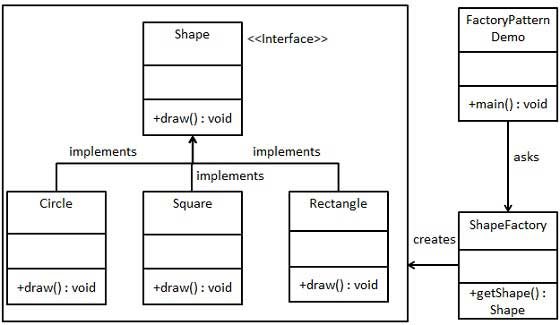
\includegraphics[scale=0.5]{Images/fact.jpg}
		\label{s1}
   		\caption{Structure du Factory Pattern}
	\end{minipage}
	
\end{figure}

\subsection{Discussions}

Ce pattern permet d'avoir plusieurs constructeurs (prenant d'autres arguments pour créer le même objet par exemple) regroupés dans une seule et même méthode factory.
Il permet d'instancier des objets dont le type est dérivé d'un type abstrait. La classe exacte de l'objet n'est donc pas connue par l'appelant.
Il est très souvent utilisé, comme par exemple la méthode java.awt.Color.make\_RGB\_color(r,g,b).



%------------------------------------


\section{Abstract Factory}
\subsection{Problématique}
\begin{itemize}
    \item Catégorie : Creational Pattern
    \item Problème : Créer des familles d'objets dépendants grâce à une même classe sans déterminer concrètement leur classe 
    \item Solution : Une "super Factory" qui crée d'autres Factories. Une interface est responsable de créer une usine à fabriquer des objets ayant des liens entre eux sans spécifier explicitement leurs classes. Chaque Factory peut retourner un nouvel objet (comme pour le Factory Pattern).
\end{itemize}
\subsection{Implémentation}
\begin{enumerate}
    \item Créer une abstract class (ou interface) AbstractFactory regroupant toutes les Factories d'objets qu'on veut créer
    \item Créer nos Factories implémentant AbstractFactory comme expliqué dans le Factory Pattern
    \item Créer une classe « FactoryProducer » qui selon l’argument appelle une autre factory qui elle va créer l’objet. Renvoie ensuite l’objet créé
    \item Créer le client dans lequel on utilise le FactoryProducer pour créer un AbstractFactory spécifique afin que le Factory concret crée l’objet qu’on veut
\end{enumerate}

\newpage
Exemple d'appel client: 
\begin{lstlisting}
    //get shape factory
  AbstractFactory shapeFactory = FactoryProducer.getFactory("SHAPE");

   //get an object of Shape Circle
  Shape shape = shapeFactory.getShape("CIRCLE");

   //call draw method of Shape Circle
  shape.draw();
\end{lstlisting}


\begin{figure}[!ht]
	\centering
	\begin{minipage}[t]{8.0cm}
		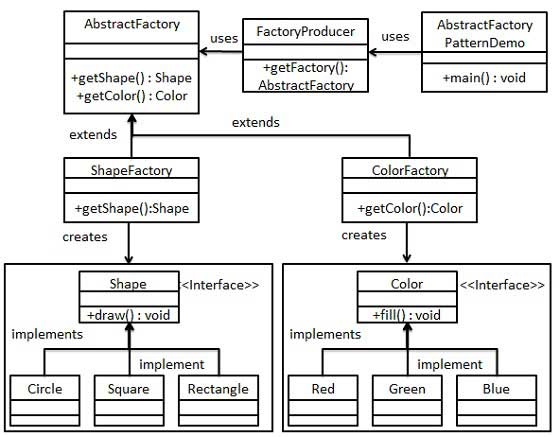
\includegraphics[scale=0.5]{Images/afact.jpg}
		\label{s1}
   		\caption{Structure de Abstract Factory Pattern}
	\end{minipage}
	
\end{figure}


\subsubsection{Discussions}
Avantage: Réduit	fortement	la	dépendance	sur	les	différentes	familles : seul	le module qui crée 
l'objet	Factory dépend des familles. \\
Inconvénient:L'objet Factory doit être transmis à tous les modules qui créent des objets de la famille. \\

Pour différencier Factory Method et Abstract Factory, on peut le voir comme ceci: le premier cache la construction d'un simple objet dans une méthode, alors que le deuxième cache la construction de toute une famille d'objets corrélés.  


%------------------------------------
\newpage
\section{Singleton}
\subsection{Problématique}
\begin{itemize}
    \item Catégorie : Creational Pattern
    \item Problème : On veut créer une classe avec une seule instance, globalement accessible.
    \item Solution : Créer et donner accès à une seule instance. Empêcher la création d'autres instances (constructeur privé).
\end{itemize}
\subsection{Implémentation}
\begin{enumerate}
    \item Créer la classe Singleton, avec le \textit{constructeur privé}, un attribut singleton = new Singleton() et une méthode getSingleton()
    \item Créer le client qui appelle getSingleton()

\end{enumerate}

\begin{figure}[!ht]
	\centering
	\begin{minipage}[t]{8.0cm}
		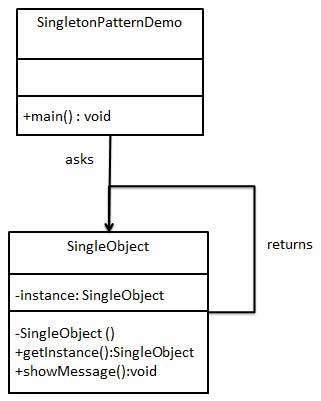
\includegraphics[scale=0.45]{Images/sing.jpg}
		\label{s1}
   		\caption{Structure du Singleton}
	\end{minipage}
	
\end{figure}


\subsection{Discussions}
Pratique pour créer un objet unique, et séparer ce code du reste du code par souci de clarté.





%------------------------------------






\section{FlyWeight }
\subsection{Problématique}
\begin{itemize}
    \item Catégorie : Structural Pattern
    \item Problème : Supporter un très grand nombre d'objets identiques (immutables). 
    \item Solution : Partager un seul objet pour toutes les instances identiques. Utiliser une méthode fabrique pour générer les instances. Distinguer l'état intrinsèque (immutable, invariable, stocké dans l'objet) et l'état extrinsèque (mutable, variable, passé en paramètre aux méthodes). 
\end{itemize}
\subsection{Implémentation}
\begin{enumerate}
    \item Créer une interface et une classe concrète l'implémentant 
    \item Créer une classe contenant une méthode Factory possédant un HashMap comme attribut: si l’objet avec la propriété passée en argument (= état immutable) n’existe pas encore, créer un nouvel objet et le renvoyer. Sinon, renvoyer un objet déjà créé en changeant uniquement son état extrinsèque.

\end{enumerate}

\begin{figure}[!ht]
	\centering
	\begin{minipage}[t]{8.0cm}
		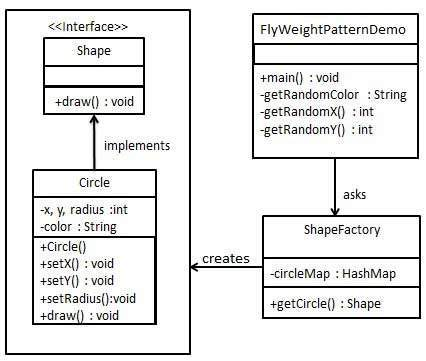
\includegraphics[scale=0.5]{Images/fly.jpg}
		\label{s1}
   		\caption{Exemple d'arborescence de FlyWeight Pattern}
	\end{minipage}
	
\end{figure}


\subsection{Discussions}
Il faut obligatoirement que l'objet ait un état intrinsèque, faute de quoi le pattern ne fonctionnera pas.
Exemple d'utilisation réelle: les String en Java.




%------------------------------------






\section{Composite}
\subsection{Problématique}
\begin{itemize}
    \item Catégorie : Structural Pattern
    \item Problème : Traiter un groupe d’objets de manière similaire à un unique objet
    \item Solution : Créer une classe contenant un groupe de ses propres objets. Cette classe fournit des manières de modifier ses groupes de mêmes objets. 
\end{itemize}
\subsection{Implémentation}
\begin{enumerate}
    \item Créer une classe Component dans laquelle il y a une liste d’instances de cette même classe. Cela permet également de représenter une forme de hiérarchie (ex : patron responsable de ("possédant") plusieurs employés, qui peuvent eux-même être responsable de ("posséder") plusieurs employés)
    \item ???
    \item Profit
\end{enumerate}

\begin{figure}[H]
	\centering
	\begin{minipage}[t]{8.0cm}
		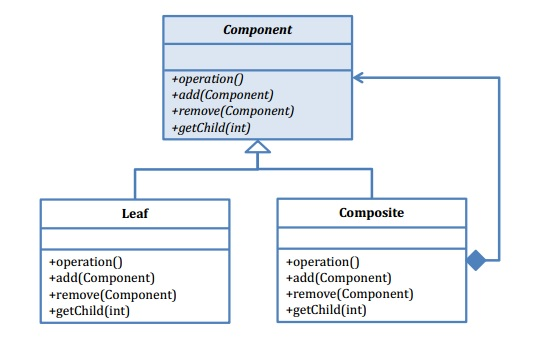
\includegraphics[scale=0.57]{Images/comp.jpg}
		\label{s1}
   		\caption{Structure de Composite Pattern}
	\end{minipage}
	
\end{figure}


\subsection{Discussions}
Permet de Simplifier les clients, car les composants primitifs et les conteneurs sont traités de la même manière.
On peut facilement ajouter des nouveaux types de composants.
Permet de maximiser les opérations offertes sur Component.





%------------------------------------





\section{Strategy}
\subsection{Problématique}
\begin{itemize}
    \item Catégorie : Behavioral Pattern
    \item Problème : Définir une famille de procédures encapsulées et interchangeables pour une fonctionnalité donnée, autrement dit donner la possibilité au code de choisir lui même l'algorithme d'exécution et/ou le comportement d'une classe.
    \item Solution : Une interface avec une méthode ayant un argument correspondant à la procédure choisie
\end{itemize}
\subsection{Implémentation}
\begin{enumerate}
    \item Créer une interface Strategy avec la méthode doOperation()
    \item Créer les classes concrètes implémentant Strategy avec des stratégies différentes (exemple: OperationAdd , OperationSubstract, OperationMultiply)
    \item Créer une classe Context qui prend une stratégie en argument dans son constructeur et possède une méthode executeStrategy()
    \item Créer le client qui n’a qu’à créer une instance de Context avec la stratégie qu’il veut en argument, puis exécuter la stratégie 

\end{enumerate}
Exemple de client : 
\begin{lstlisting}
    Context context = new Context(new OperationAdd());		
    System.out.println("10 + 5 = " + context.executeStrategy(10, 5));
\end{lstlisting}


\begin{figure}[H]
	\centering
	\begin{minipage}[t]{8.0cm}
		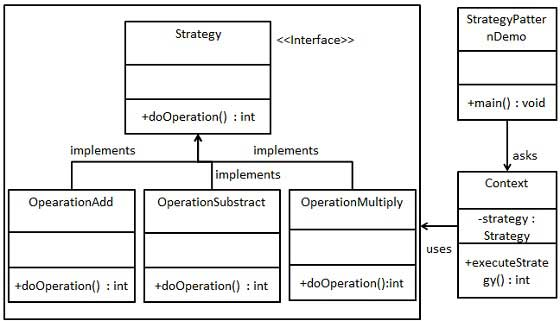
\includegraphics[scale=0.4]{Images/strat.jpg}
		\label{s1}
   		\caption{Exemple d'arborescence du Strategy Pattern}
	\end{minipage}
	
\end{figure}


\subsection{Discussions}
L'utilité de ce pattern est de séparer des algorithmes différents dans différentes classes qui pourront être choisis et exécutés au moment de l'exécution, en plus de garder une clarté dans le code.
Un exemple très connu est la méthode compareTo() dans Object en Java.





%------------------------------------




\section{Command}
\subsection{Problématique}
\begin{itemize}
    \item Catégorie : Behavioral Pattern
    \item Problème : Définir une famille de requêtes encapsulées et interchangeables pour des comportements quelconques 
    \item Solution : Une interface avec une méthode correspondant à la requête
\end{itemize}
\subsection{Implémentation}
\begin{enumerate}
    \item Créer une interface Commande (Order) qui ne possède que quelques méthodes (execute() au minimum; undo() et redo() sont aussi généralement utilisées)
    \item Créer une classe concrète Receiver qui correspond à l’objet qui subira la commande/l’action (exemples: télévision, document)
    \item Créer des classes concrètes implémentant Commande, chacune représentant une commande particulière dépendant du Receiver (exemples:: télévision : on/off/volumeUp/volumeDown ; document : save/open )
    \item Créer une classe Invoker, qui possède une liste de commandes et peut soit en rajouter soit les exécuter (la liste n'est pas obligatoire mais permet de retenir les commandes et donc d'implémenter les undo/redo)
    \item Créer la classe Client, qui instancie des nouvelles commandes, peut les rajouter à la liste du Invoker et les exécuter quand il veut.

\end{enumerate}
\newpage
Exemple d'appel de client: 
\begin{lstlisting}
    Television tv = new Television();

    TvOn tvOnOrder = new TvOn(tv);
    TvVolumeUp tvUpOrder = new TvVolumeUp(tv);
    
    Invoker button = new Invoker();
    button.takeOrder(tvOnOrder);
    button.takeOrder(tvUpOrder);
    
    button.executeOrders();
\end{lstlisting}


\begin{figure}[H]
	\centering
	\begin{minipage}[t]{8.0cm}
		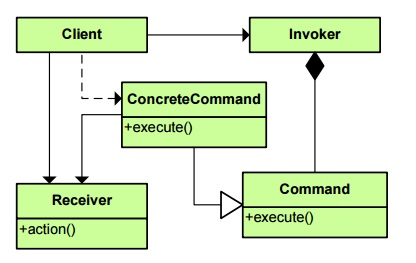
\includegraphics[scale=0.7]{Images/comm.jpg}
		\label{s1}
   		\caption{Structure de Command Pattern}
	\end{minipage}
	
\end{figure}

\subsection{Discussions}

La commande n'a pas de résultat mais produit un effet. Les données du contexte sont fournies à la construction de la commande. Permet d'éviter des conditionnelles. Les commandes peuvent être postposées, mises en files, transférées, rejouées, … Supporte undo avec une méthode supplémentaire



%------------------------------------






\section{Observer}
\subsection{Problématique}
\begin{itemize}
    \item Catégorie : Behavioral Pattern
    \item Problème : Définir un lien entre objets tel que quand un objet est modifié, les objets dépendants soient notifiés. 
    \item Solution : C'est le sujet qui invoque observer.update() dans une méthode notifyChanges(), au lieu de l'observer qui vient demander si un changement a été apporté
\end{itemize}
\subsection{Implémentation}
\begin{enumerate}
    \item Créer une interface Observer contenant la méthode update() et les classes concrètes l'implémentant
    \item Créer l’interface Subject contenant 3 méthodes : attach() / detach() ( = s'abonner ou se désabonner aux notifications) et notify() (appelle les méthodes update() de tous les observers abonnés)
    

\end{enumerate}

\begin{figure}[!ht]
	\centering
	\begin{minipage}[t]{8.0cm}
		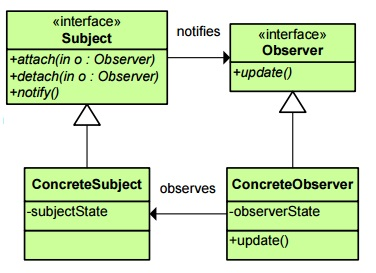
\includegraphics[scale=0.7]{Images/obs.jpg}
		\label{s1}
   		\caption{Structure de Observer Pattern}
	\end{minipage}
	
\end{figure}


\subsection{Discussions}
Ce pattern est beaucoup utilisé pour tout ce qui est interaction avec l'interface graphique (boutons, editTexts, etc.). Il permet de gagner du temps et de la mémoire, car sans cette méthode, les observateurs devraient vérifier toutes les x secondes si un changement a été apporté. \\
Voici un exemple concret pour mieux comprendre ce pattern. Considérer le subject comme un reporter freelance ayant pour rôle de dénicher des scoops et les Observers comme des grandes chaînes de télévision (Rtbf, RTL, ...). Le principe du pattern est que lorsqu'il a un scoop, le reporter prévient toutes les chaînes qui le paient pour avoir des scoops. Or sans ce pattern, les chaînes ne cesseraient d'appeler le reporter pour demander s'il y a du nouveau, ce qui est une grande perte de temps pour les deux partis.






%------------------------------------






\section{Interpreter}
\subsection{Problématique}
\begin{itemize}
    \item Catégorie : Behavioral Pattern
    \item Problème : Définir un calcul sur une structure arborescente (représentant les phrases d'un langage). Convertir une représentation de données en une autre représentation des mêmes données. Parcourir un arbre d’interprétation en effectuant un certain calcul (Plusieurs calculs différents (évaluer, imprimer, …) + le calcul dépend du type de noeud )
    \item Solution : Une méthode interpret sur toutes les classes de l'arborescence + TerminalExpression (=leaf) et CompoundExpression(= noeud)
\end{itemize}
\subsection{Implémentation}
\begin{enumerate}
    \item Créer une classe abstraite (ou interface) Expression contenant une méthode interpret()
    \item Créer des classes terminales TerminalExpression implémentant Expression, attribuant une valeur finale (leaf) à l’expression passée en argument. Ces classes permettent de traiter les plus petits morceaux de l'information reçue (si on a par exemple (a \&\& b) comme entrée, les deux 'leaves' ou plus petites parties sont a et b, et TerminalExpression.interpret(a) devrait renvoyer true si a==true et false sinon )
    \item Créer d’autres classes implémentant Expression, toutes composites (voir le Design Pattern Composite) et appelant les méthodes interpret() de chaque expression (en continuant dans le même exemple, on pourrait par exemple avoir OrExpression ou AndExpression)
    \item Créer les classe concrètes Client et Contexte (dans l'exemple ci-dessus le contexte serait des Boolean).

\end{enumerate}

\begin{figure}[!ht]
	\centering
	\begin{minipage}[t]{8.0cm}
		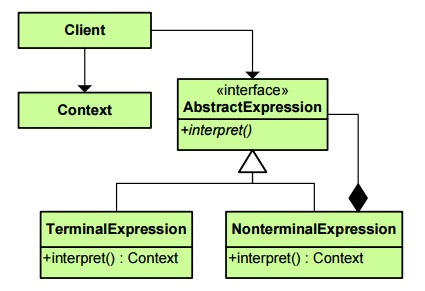
\includegraphics[scale=0.65]{Images/int.jpg}
		\label{s1}
   		\caption{Structure de Interpreter Pattern}
	\end{minipage}
	
\end{figure}


\subsection{Discussions}
Ce pattern est basé sur le patron Composite et est le plus souvent utilisé pour interpréter un langage, mais il reste applicable à tout autre type de structure composée. Il permet l'extension facile d'un langage ou l'ajout de fonctions d'interprétation difficiles (une méthode par classe du langage). Egalement utilisé lorsqu’un logiciel doit analyser/parser une chaîne algébrique (= expression) ou lorsqu’un logiciel doit produire différents types de données comme résultat.




%------------------------------------






\section{Visitor}
\subsection{Problématique}
\begin{itemize}
    \item Catégorie : Behavioral Pattern
    \item Problème : Définir plusieurs calculs basée sur une seule structure, sans changer les classes de la structure. Séparer un algorithme d’une structure de données
    \item Solution : ElementA.accept(v) appelle visitElementA(this)
\end{itemize}
\subsection{Implémentation}
\begin{enumerate}
    \item Créer une interface Visitable (ou Element) contenant la méthode accept(Visitor v)
    \item Créer les classes concrètes implémentant Visitable, les méthodes accept() faisant appel à v.visit(this)
    \item Créer une interface Visitor contenant toutes les méthodes visit(Visitable v)
    \item Créer une classe ConcreteVisitor implémentant Visitor et toutes ses méthodes

\end{enumerate}



\begin{figure}[!ht]
	\centering
	\begin{minipage}[t]{8.0cm}
		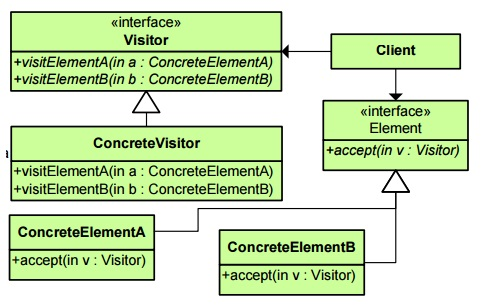
\includegraphics[scale=0.65]{Images/vis.jpg}
		\label{s1}
   		\caption{Structure de Visitor Pattern}
	\end{minipage}
	
\end{figure}


\subsection{Discussions}
Ce pattern est très pratique lorsqu’on veut ajouter une fonctionnalité sans trop modifier le code de base par souci de clarté (exemple: le débuggage). Il peut s'appliquer à toute structure, pas uniquement les Composite. On peut mettre le parcours de la structure dans le visiteur. On a un parcours plus précis en fonction du calcul (+++), mais répété pour chaque visiteur (---).



\newpage
\part{Annexes}




% Please add the following required packages to your document preamble:

\begin{sidewaystable}[]
\centering
\caption{\large{Design Patterns en un coup d'oeil}}
\label{my-label}
\begin{tabular}{|c|c|l|}
\hline
\textit{\textbf{Pattern}} & \textit{\textbf{Type}}    & \multicolumn{1}{c|}{ \textit{\textbf{A utiliser dans le cas où:}}}                                                                                                                                                                                                                                                                                                                                     \\ \hline
\textbf{Factory method}         & Creationnal                     & \begin{tabular}[c]{@{}l@{}}On veut que client ne sache pas quelles classes sont nécessaires pour créer l'objet voulu\\ On veut que soient les sous-classes qui décident quels objets doivent être créer\\ La création d'un objet ne peut pas être géré pas les classes parents\end{tabular}                                                                                                                                                                  \\ \hline
\textbf{Abstract Factory}       & Creationnal                     & \begin{tabular}[c]{@{}l@{}}Le processus création d'objets doit être indépendant de celui de leur utilisation\\ Les systèmes doivent être capables d'utiliser plusieurs familles d'objets\\ Des familles d'objets doivent être utilisés ensemble (dans des listes par exemple)\\ Le client ne peut pas savoir quelles classes sont nécessaires pour créer l'objet voulu\end{tabular}                                                                          \\ \hline
\textbf{Singleton}              & Creationnal                     & \begin{tabular}[c]{@{}l@{}}Il ne peut exister qu'une unique instance de la classe\\ L'accès à cet unique instance doit êtrecontrôlé.\end{tabular}                                                                                                                                                                                                                                                                                                            \\ \hline
\textbf{FlyWeight}              & Structural                      & \begin{tabular}[c]{@{}l@{}}De nombreux objets semblables doivent être utilisés et leur coût en mémoire est élevé\\ La majorité des états de ces objets peut être rendu intrinsèque (immutable)\\ Un petit nombre d'objets partagés peuvent remplacer un grand nombre de non partagés\\ L'identité de chaque objet n'a pas d'importance\end{tabular}                                                                                                          \\ \hline
\textbf{Composite}              & Structural                      & \begin{tabular}[c]{@{}l@{}}On a besoin d'une représentation hiérarchique (pas besoin de connaître tout l'arbre)\\ Les objets et les regroupements d'objets doivent être traités de la même manière\end{tabular}                                                                                                                                                                                                                                              \\ \hline
\textbf{Strategy}               & Behavioral                      & \begin{tabular}[c]{@{}l@{}}La seule différence entre plusieurs classes reliées est leurs comportements\\ De multiples versions/variations d'un même algorithmes sont nécessaires\\ L'accès aux algorithmes et l'utilisation des données qu'ils utilisent ne doivent pas être exposés\\ Le comportement d'une classe doit être défini lors de l'exécution uniquement\\ Les expressions conditionnelles sont complexes et compliquées à maintenir\end{tabular} \\ \hline
\textbf{Command}                & \multicolumn{1}{l|}{Behavioral} & \begin{tabular}[c]{@{}l@{}}On a besoin d'une fonctionnalité "retour en arrière"/ d'un historique des requêtes\\ Les requêtes doivent être traitées dans des ordres différents\\ L'invocateur doit être dissocié des l'objet s'occupant de l'invocation\end{tabular}                                                                                                                                                                                          \\ \hline
\textbf{Observer}               & \multicolumn{1}{l|}{Behavioral} & \begin{tabular}[c]{@{}l@{}}Le changement d'état d'un ou plusieurs objet doit activer certains comportements dans d'autres objets\\ La diffusion (d'informations) est nécessaire\end{tabular}                                                                                                                                                                                                                                                                 \\ \hline
\textbf{Interpreter}            & \multicolumn{1}{l|}{Behavioral} & \begin{tabular}[c]{@{}l@{}}Il faut interpréter de la grammaire qui peut être représentée comme des arbres de syntaxe larges\\ La grammaire est simple\\ Le rendement n'est pas primordial\end{tabular}                                                                                                                                                                                                                                                       \\ \hline
\textbf{Visitor}                & \multicolumn{1}{l|}{Behavioral} & \begin{tabular}[c]{@{}l@{}}De nombreuses opérations n'ayant aucun lien avec une structure d'objet doivent être réalisées\\ La structure ne peut pas changer mais les opérations bien\\ Les opérations doivent fonctionner sur de multiples structures d'objets implémentant les mêmes interfaces\end{tabular}                                                                                                                                                \\ \hline
\end{tabular}
\end{sidewaystable}
\end{document}
